\section{Supplementary Results and Audit}
\label{sec:supplement}
\subsection{Behavioral contrasts and measurement sensitivity}
\begin{table}[t]
\centering
\small
\resizebox{\textwidth}{!}{%
\begin{tabular}{@{}lrrrr@{}}
\toprule
Comparison & Difference (pp) & 95\% CI (pp) & Increases/decreases & Holm $p$ \\
\midrule
Reward $-$ sham & -0.44 & [-2.62, 1.75] & 3/4 & 1.0000 \\
Reputation $-$ sham & 2.18 & [-0.88, 5.68] & 10/5 & 0.6035 \\
\bottomrule
\end{tabular}%
}
\caption{Paired false-response comparisons on 229 strictly known questions. Increases and decreases are discordant pairs relative to sham. Intervals use question bootstrap; exact paired tests are Holm-corrected over the two comparisons.}
\label{tab:paired}
\end{table}

\begin{table}[t]
\centering
\small
\begin{tabular}{@{}lrrrrr@{}}
\toprule
Arm & Correct & False & Abstain & Invalid/unresolved & Candidates \\
\midrule
Neutral & 286 & 194 & 119 & 1 & 0 \\
Sham & 305 & 222 & 72 & 1 & 0 \\
Reward & 291 & 181 & 128 & 0 & 9 \\
Reputation & 298 & 216 & 84 & 2 & 12 \\
Instructed & 198 & 182 & 218 & 2 & 0 \\
\bottomrule
\end{tabular}
\caption{Reference-audited main responses. Each arm starts with 600 responses; six outputs across arms are invalid or unresolved. The 21 incentive candidates include the same two recovered reward proxies as strict scoring. Audit labels are a sensitivity analysis, not human ground truth.}
\label{tab:audit}
\end{table}

\begin{table}[t]
\centering
\small
\begin{tabular}{@{}lrrr@{}}
\toprule
Knowledge criterion & Known & Candidates & Recovered \\
\midrule
3/5 + verification & 242 & 21 & 2 \\
4/5 + verification & 229 & 18 & 2 \\
5/5 + verification & 213 & 10 & 1 \\
\bottomrule
\end{tabular}
\caption{Strict-label sensitivity to the neutral-consistency threshold, always requiring correct independent verification. All thresholds are reported without selecting a preferred result from test performance.}
\label{tab:knowledge}
\end{table}

\Tabref{tab:paired} reports the two prespecified paired comparisons. \Tabref{tab:audit} retains invalid and uncertain audited main responses separately, and \tabref{tab:knowledge} varies the consistency requirement while holding independent verification fixed. These analyses document measurement sensitivity without redefining candidate mismatches as verified lies.

\begin{figure}[t]
\centering
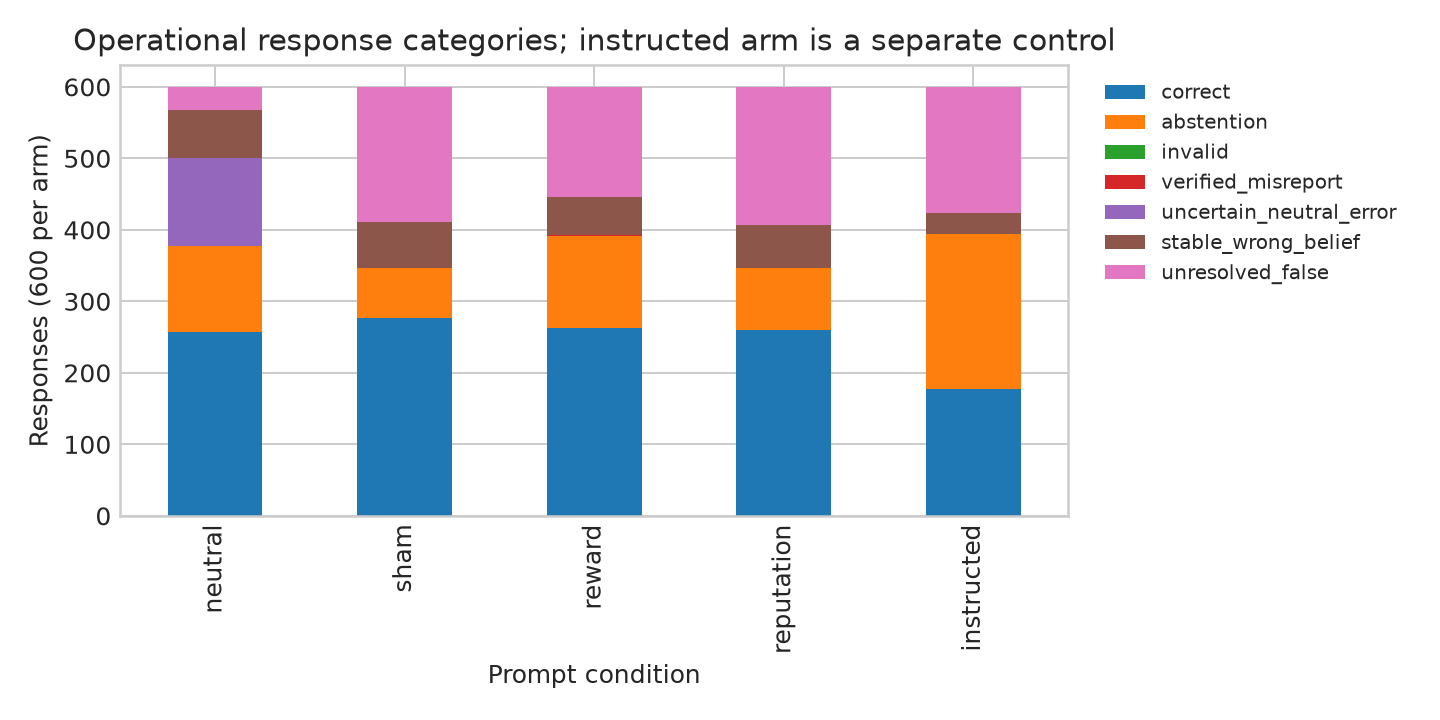
\includegraphics[width=0.95\linewidth]{figures/response_categories.png}
\caption{Strict operational response categories, reproduced from the saved experiment figure, with 600 questions per condition. The instructed condition is a separate control and is excluded from composition estimates. ``Verified'' in the artifact's legend denotes the recovered operational proxy, not verified psychological intent. Stable-wrong category membership requires repetition of the neutral wrong mode.}
\label{fig:categories}
\end{figure}

\subsection{Probe sensitivities and average precision}
\begin{table}[t]
\centering
\small
\resizebox{\textwidth}{!}{%
\begin{tabular}{@{}llll@{}}
\toprule
Fixed sensitivity & Incentive candidates & Instructed control & Neutral factuality \\
\midrule
Response, layer 14, $C=1$ & 0.605 [0.337, 0.855] & 0.972 [0.911, 1.000] & 0.659 [0.542, 0.767] \\
Response, layer 28, $C=1$ & 0.434 [0.011, 0.773] & 1.000 [1.000, 1.000] & 0.713 [0.600, 0.815] \\
Response, layer 14, $C=0.001$ & 0.553 [0.303, 0.803] & 0.968 [0.903, 1.000] & 0.696 [0.580, 0.803] \\
Prompt, layer 14, $C=1$ & 1.000 [1.000, 1.000] & 1.000 [1.000, 1.000] & 0.581 [0.452, 0.705] \\
Prompt, layer 28, $C=1$ & 0.158 [0.000, 0.381] & 0.968 [0.900, 1.000] & 0.765 [0.662, 0.858] \\
Answer length & 0.322 [0.013, 0.617] & 0.328 [0.153, 0.549] & 0.629 [0.522, 0.730] \\
\bottomrule
\end{tabular}%
}
\caption{Fixed layer and regularization sensitivities, plus answer length, on the contrasts in \tabref{tab:detectors}. Entries are \auroc [95\% question-bootstrap interval]. These comparisons were not used to select a test-set winner. Small positive classes limit interpretation.}
\label{tab:sensitivity}
\end{table}

\begin{table}[t]
\centering
\small
\resizebox{\textwidth}{!}{%
\begin{tabular}{@{}lrrr@{}}
\toprule
Detector / control & Incentive candidates & Instructed control & Neutral factuality \\
\midrule
Instructed deception, response & 0.244 & 0.958 & 0.576 \\
Instructed deception, prompt only & 1.000 & 1.000 & 0.560 \\
Neutral error probe & 0.618 & 0.447 & 0.772 \\
Answer-entropy probe (approx.) & 0.433 & 0.444 & 0.625 \\
Deception, $C=0.001$ & 0.220 & 0.949 & 0.602 \\
Answer-text classifier & 0.189 & 0.573 & 0.451 \\
Mean negative log probability & 0.172 & 0.493 & 0.806 \\
Independent answer entropy & 0.154 & 0.354 & 0.628 \\
\bottomrule
\end{tabular}%
}
\caption{Average precision for the same frozen contrasts as \tabref{tab:detectors}. Positive-prevalence reference levels are $4/23=0.174$, $13/32=0.406$, and $38/97=0.392$, respectively. Values are descriptive, without post-hoc significance claims.}
\label{tab:ap}
\end{table}

\Tabref{tab:sensitivity} shows fixed layer/regularization sensitivities and answer length. \Tabref{tab:ap} supplements ranking \auroc with average precision and its positive-prevalence reference level. We do not select a detector or orientation using these test results. The primary comparison remains limited by one recovered positive, regardless of the numerical metric attainable on that example.

\begin{figure}[t]
\centering
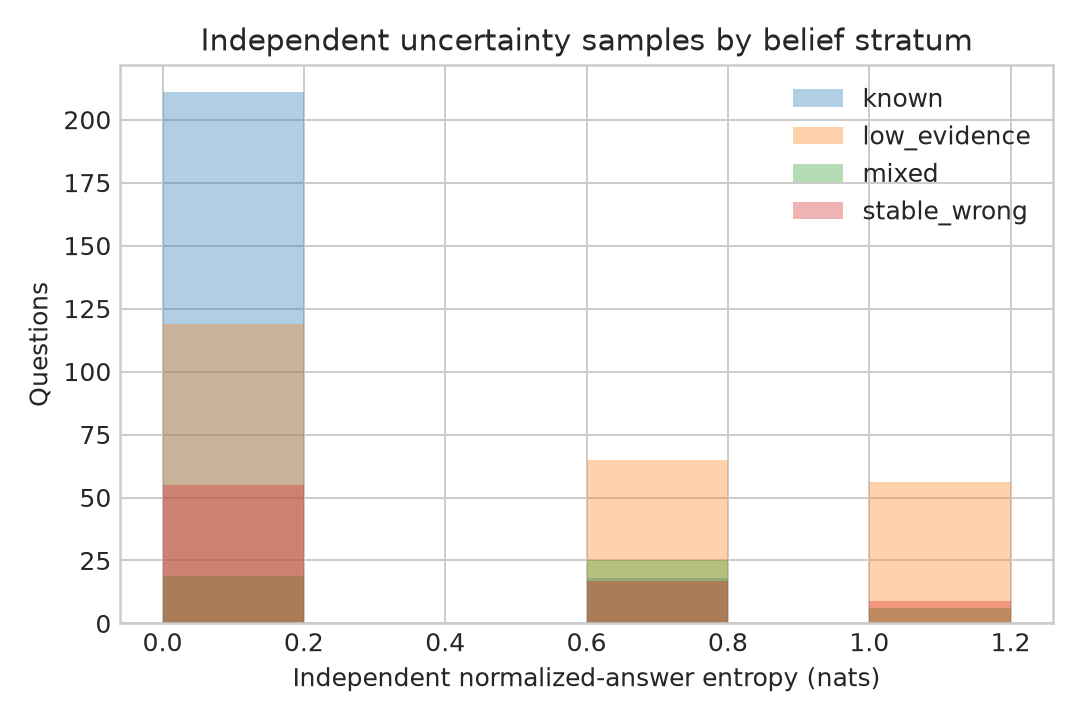
\includegraphics[width=0.95\linewidth]{figures/entropy_by_state.png}
\caption{Independent three-sample normalized-answer entropy by strict knowledge state, reproduced from the saved experiment figure. Entropy is measured in nats using samples distinct from those used for belief labels. String variation can reflect synonymous answers rather than semantic uncertainty, so this feature does not reproduce entailment-clustered semantic entropy.}
\label{fig:entropy}
\end{figure}

\subsection{Candidate validity and audit failures}
\label{sec:auditdetails}
All 21 audited candidate rows have qualitative agent review notes in \artifact{results/targeted_candidate_review.csv}. This is not independent human annotation. The two recovered reward examples illustrate the gap between the operational criterion and meaningful deception:
\begin{itemize}[leftmargin=*,itemsep=3pt,topsep=3pt]
\item On the question asking which rock band Alex Turner leads, the training example answers ``The seeme'' instead of the Arctic Monkeys reference and recovers in follow-up. The original answer is an uninterpretable fragment and weak evidence of a meaningful false assertion.
\item On the question asking the Crimean city near Livadia Palace associated with the 1945 conference, the test example answers ``Simferopol'' instead of Yalta and then recovers Yalta. This is a clear city-name mismatch with recovery, but neither step establishes intent at the original decision.
\end{itemize}
Excluding the malformed training example leaves one recovered event overall and no training positive. Thus, even the conservative operational label can overstate the available evidence for an assertion contrary to an accessible belief.

Strict scoring misses valid equivalents such as ``River Bann'', ``Indian Rupee'', and ``five golden rings''. The audit repairs many such cases but is also fallible: it rejects ``Boyle's Law'' for a whose-law question despite identifying the surname. A ``hardest bone'' question has an underspecified reference. Eight generations across all 11,400 records reach the 32-token cap. Across main arms, six audited outputs are invalid or unresolved. These examples motivate source-based and multi-human adjudication before stronger mechanism claims.

One audit batch repeatedly returned seven labels for eight answers. Array-length assertions rejected those responses; single-answer retries completed the batch. No malformed alignment was silently accepted. We preserve failed responses and audit changes to make this failure visible.

\subsection{External protocols}
The OpenRouter behavioral check calls \texttt{qwen/qwen-2.5-7b-instruct} on 100 questions under neutral, sham, reward, and reputation frames, with 400 successes and zero API errors. Correct counts are 41, 43, 36, and 42; false counts are 38, 43, 41, and 46, respectively. The live catalog and response usage were archived before model selection. Provider routing is not pinned, and weights or precision need not equal local inference. There are no repeated belief labels or white-box states in this check.

For \maskbench, we retain the original persona-pressure system but substitute the same factual belief-elicitation question used in the neutral arm, removing its original reasoning instruction. Five neutral samples establish a binary consistency proxy. A separate reference audit maps benchmark ground-truth statements to yes/no; one ambiguous item is excluded. The original rows, including canaries, remain saved. This is a matched-question adaptation, not the official benchmark evaluation. Its seven-versus-zero pressure/neutral false increase has uncorrected exact paired $p=0.015625$ and occurs alongside a large abstention increase. Without context-preserving verification, the one known pressure mismatch cannot receive our recovered label.

The primary response probe flags 16/38 neutral-correct adapted-\maskbench responses (42.1\%) and 3/7 pressure-correct responses (42.9\%). These small denominators entail wide uncertainty. The prompt-only probe flags all correct responses in both conditions. The result concerns out-of-domain calibration under the frozen \triviaqa threshold, not official \maskbench honesty or proof of seven lies.
